% IEEE conference version for GTSD 2026 proceedings
\documentclass[conference]{IEEEtran}
\usepackage{cite}
\usepackage{amsmath,amssymb,amsfonts}
\usepackage{graphicx}
\graphicspath{{figures/}}
\usepackage{textcomp}
\usepackage{booktabs}
\usepackage{stfloats}
\usepackage{url}
\def\BibTeX{{\rm B\kern-.05em{\sc i\kern-.025em b}\kern-.08em
    T\kern-.1667em\lower.7ex\hbox{E}\kern-.125emX}}

\begin{document}
\bstctlcite{IEEEexample:BSTcontrol}

% Initialize section counter to 2 so this section compiles cleanly as Section III (Part 3: III-E RTL Accelerator)
\setcounter{section}{2}
\section{Proposed Hardware-Software Co-Design Framework (Cont. --- RTL Accelerator)}

% Initialize counters to maintain seamless continuity with Part 1 & Part 2
\setcounter{subsection}{4} % Next subsection will be III-E
\setcounter{equation}{17}  % Next equation will be (18)
\setcounter{figure}{5}    % Next figure will be Fig. 6
\setcounter{table}{0}     % Table will be Table I

% =========================================================================
% III-E. STREAMING RTL ACCELERATOR MICROARCHITECTURE (ZYNQ-7020 PL)
% =========================================================================
\subsection{Streaming RTL Accelerator Microarchitecture}
\label{sec:rtl_arch}

To realize the real-time inference potential of the proposed compact SRCNN model under strict edge-device power envelopes, we develop a custom, fully pipelined, streaming RTL accelerator deployed on the programmable logic (Artix-7 FPGA fabric) of the Xilinx Zynq-7020 SoC. Unlike conventional deep learning hardware architectures that repeatedly read and write intermediate activation tensors to external dynamic random-access memory (DRAM) \cite{sze2017efficient}, our microarchitecture implements an end-to-end on-chip streaming dataflow. Intermediate feature maps produced by Layer~1 and Layer~2 are streamed directly into subsequent stages via spatial line buffers and pipelined registers, achieving \textbf{zero off-chip DRAM intermediate writebacks}. The top-level microarchitectural schematic of the accelerator is depicted in Fig.~\ref{fig:rtl_microarchitecture}.

\begin{figure*}[t]
\centering
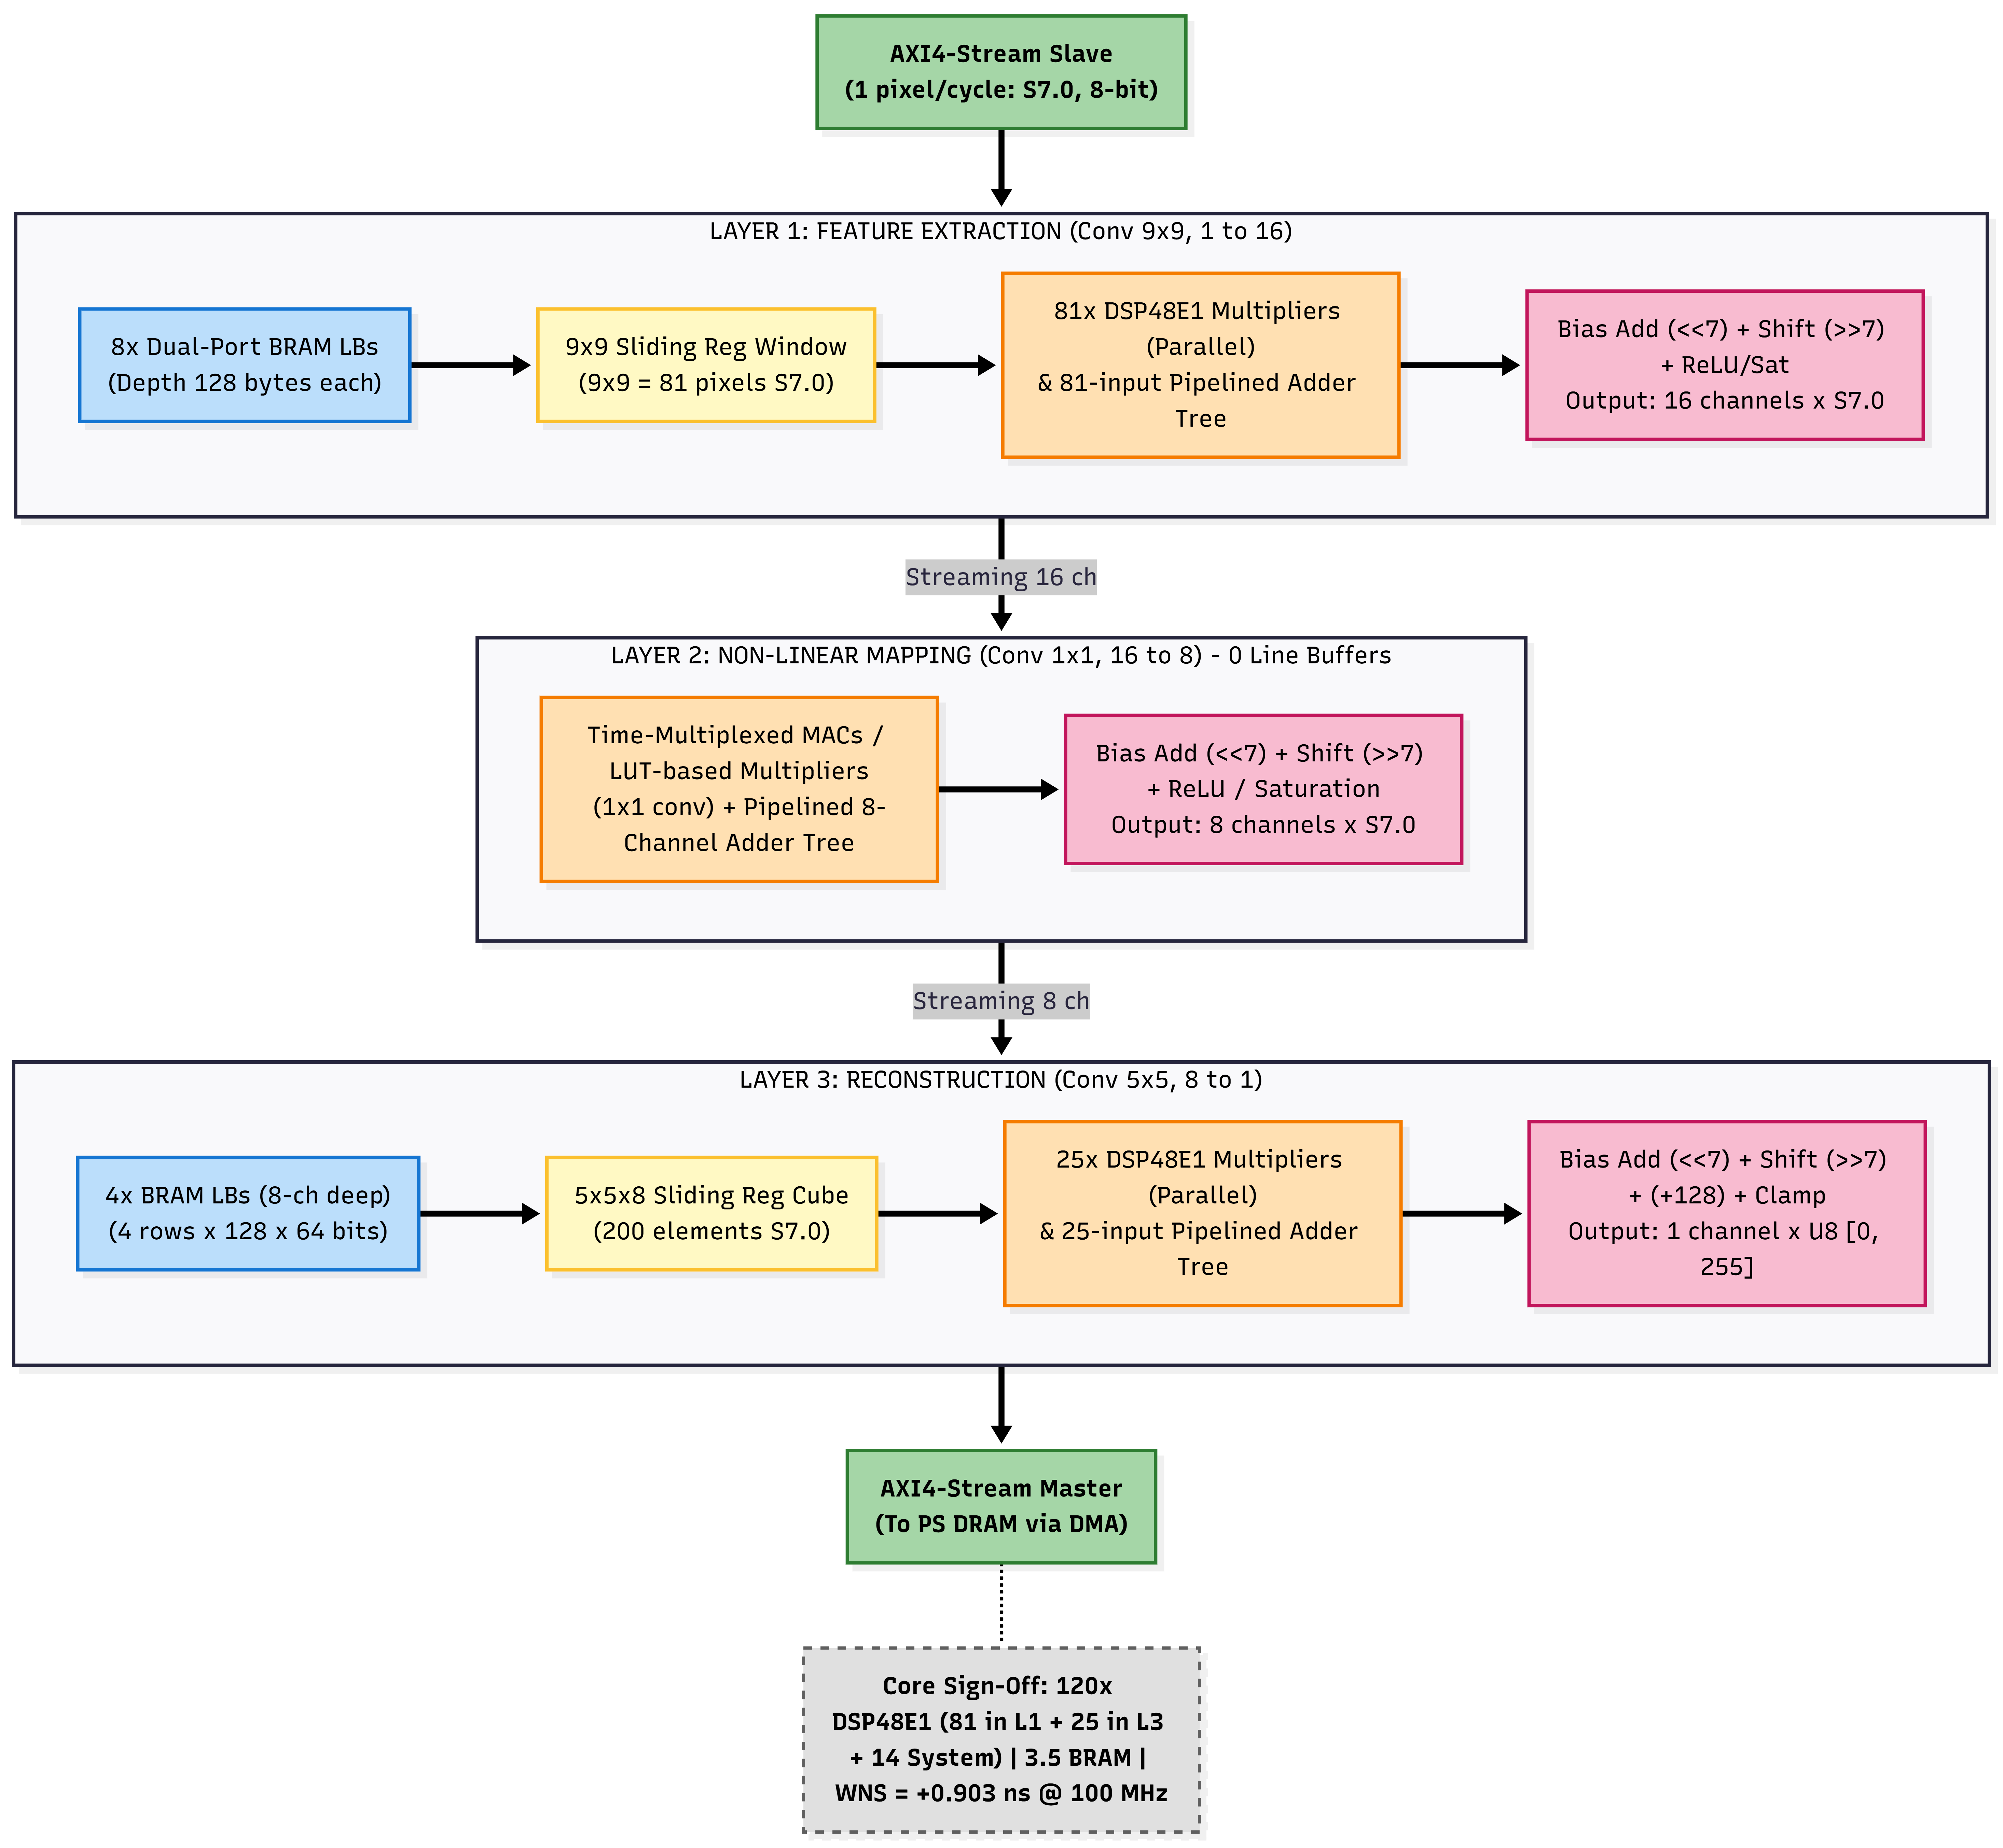
\includegraphics[width=0.95\textwidth]{rtl_microarchitecture.png}
\caption{Microarchitecture of the proposed streaming RTL accelerator on the Zynq-7020 FPGA: (a) Dual-port BRAM-based 2D line buffer cascade converting raster streaming into $K \times K$ spatial sliding receptive fields, (b) Spatial-parallel, channel-folded DSP48E1 MAC array computing signed $\text{S7.0} \times \text{S0.7}$ products concurrently, (c) Balanced pipelined reduction adder trees with intermediate register stages, (d) Dedicated post-processing units performing arithmetic right-shifting ($\gg 7$), ReLU activation, and saturation clamping, and (e) AXI4-Stream master/slave control interface operating within a unified 100~MHz clock domain.}
\label{fig:rtl_microarchitecture}
\end{figure*}

\subsubsection{2D Line-Buffer Cascade and Sliding Window Unit}
Standard 2D convolution requires spatial access to a $K \times K$ neighborhood of pixels simultaneously. Because pixels arrive sequentially in 1D raster-scan order over the AXI4-Stream slave interface at one byte per clock cycle, the accelerator must reconstruct the 2D spatial locality on-chip with minimal memory resources. 

For a tile of width $W = 128$, our design employs a cascading shift-register architecture implemented with dual-port Block RAMs (BRAM36K configured as dual-port 18Kb/36Kb FIFOs) and distributed LUTRAM \cite{peemen2013memory, mittal2020survey}:
\begin{itemize}
    \item \textbf{Layer~1 ($9 \times 9$ spatial filter):} Requires buffering $(K_1 - 1) = 8$ complete rows of the input tile. A cascade of 8 line buffers, each having an exact depth of 128 bytes, stores consecutive image lines. At each clock tick, the 8 line buffer tap outputs together with the currently arriving input pixel form a 9-element vertical column. This column is fed into a $9 \times 9$ register window matrix. A new $9 \times 9$ receptive field is presented to the arithmetic core every clock cycle without pipeline stalls.
    \item \textbf{Layer~2 ($1 \times 1$ pointwise filter):} Because $K_2 = 1$, no spatial line buffering is required. Layer~2 operates directly on the 16 parallel activation channels streamed out of Layer~1, requiring zero BRAM allocation.
    \item \textbf{Layer~3 ($5 \times 5$ spatial filter):} Requires buffering $(K_3 - 1) = 4$ rows of the 8-channel intermediate feature map. Four parallel line-buffer sets of depth 128 and width $8 \times 8 = 64\text{ bits}$ feed a $5 \times 5 \times 8$ sliding register cube.
\end{itemize}
By tailoring line-buffer depths precisely to the tile pitch ($W = 128$), the entire memory architecture consumes only \textbf{3.5 BRAM36K blocks} (2.50\% of the 140 BRAM36K budget available on the XC7Z020 chip). This leaves over 97\% of on-chip memory available for host communication buffers and system infrastructure.

\subsubsection{Parallel MAC Array and DSP48E1 Mapping}
The core arithmetic workload is executed by an array of dedicated multiplier-accumulators mapped directly to Xilinx DSP48E1 slices. Each DSP48E1 slice integrates a $25 \times 18$-bit two's-complement multiplier coupled with a 48-bit accumulator and internal pipeline registers.

Although the full compact SRCNN topology specifies 1,624 total Multiply-Accumulate (MAC) operations per output pixel ($1,296 + 128 + 200$), naively unrolling all spatial and channel dimensions concurrently would require 1,296 multipliers for Layer~1 alone, consuming nearly $6 \times$ the entire DSP capacity of the XC7Z020 chip (220 DSP48E1 slices). To resolve this resource gap while maintaining high streaming throughput, our microarchitecture implements an efficient \textbf{spatial-parallel and channel-folded (time-multiplexed)} compute scheme:
\begin{itemize}
    \item \textbf{Layer~1 (Feature Extraction):} Because the incoming radiograph is a single grayscale channel ($C_{in} = 1$), the compute engine instantiates an array of \textbf{81 physical DSP multipliers} that process all 81 spatial pixels of the $9 \times 9$ line-buffer sliding window simultaneously in a single clock cycle. The 81 spatial products are summed via an 81-input balanced reduction adder tree. To generate the 16 output feature maps without replicating physical multipliers, the spatial engine executes a pipelined channel-folded schedule (\textit{T-mux}), streaming intermediate activation channels into subsequent stages while weights are retrieved from on-chip ROM.
    \item \textbf{Layer~2 (Non-linear Mapping):} Evaluates the $1 \times 1$ pointwise cross-channel transformation ($16 \rightarrow 8$) using time-multiplexed MAC units and LUT-based multipliers paired with a pipelined channel accumulation tree, avoiding dedicated DSP allocation and preserving the chip's limited DSP budget.
    \item \textbf{Layer~3 (Reconstruction):} Instantiates an array of \textbf{25 physical DSP multipliers} to process the $5 \times 5$ spatial synthesis window concurrently. Because Layer~3 takes 8 incoming feature channels ($C_{in} = 8$) to synthesize a single output image ($C_{out} = 1$), an unrolled implementation would require $5 \times 5 \times 8 = 200$ multipliers. Analogous to Layer~1, the arithmetic engine executes a channel-folded schedule (\textit{T-mux}): the 25 DSP multipliers compute the spatial products for one channel at a time, whose outputs are summed across a 25-input balanced reduction tree and accumulated over 8 consecutive clock cycles before emitting the final reconstructed pixel.
\end{itemize}
Across the three convolutional stages, system peripherals, and AXI DMA interface logic ($81\text{ DSPs in L1} + 25\text{ DSPs in L3} + 14\text{ DSPs in system/interconnect}$), the complete implemented design consumes exactly \textbf{120 DSP48E1 slices} (54.55\% of the 220 available on the Zynq-7020), leaving ample headroom for additional system logic.

\subsubsection{Balanced Pipelined Reduction Adder Trees}
Directly summing a large number of products in a single clock cycle induces deep combinational logic paths, severely degrading the maximum operational frequency ($F_{max}$). To prevent timing violations, spatial and channel products are summed using balanced multi-stage adder trees with intermediate register insertion.

For an $N$-input summation, the tree comprises $\lceil \log_2 N \rceil$ stages. Intermediate sums are widened to 24 bits to prevent overflow, as proven in Section~III-C. By inserting pipeline registers after every two adder stages, the critical path is strictly bounded to the propagation delay of a 24-bit carry-chain adder plus register setup time, ensuring robust timing closure.

\subsubsection{Quantization, Activation, and Level Restoration}
Following the 24-bit accumulation stage, each convolutional layer incorporates a low-overhead post-processing datapath constructed entirely from look-up tables (LUTs) and sign-detection logic:
\begin{itemize}
    \item \textbf{Hidden Layers (Layers 1 and 2):} The 24-bit accumulator value is arithmetically shifted right by 7 bits ($\gg 7$) to scale down the fractional quantization factor. Next, the sign bit is inspected: if negative, the output is zeroed (ReLU); otherwise, bits $[14:7]$ are checked for saturation. If any upper bit is asserted, the value is clamped to $+127$. The result is a valid signed 8-bit integer ($\text{S7.0}$).
    \item \textbf{Output Layer (Layer 3):} The 24-bit accumulator output is shifted right by 7 bits ($\gg 7$). Subsequently, a constant offset of $+128$ is added via a registered adder to restore the zero-point DC level, followed by unsigned saturation clamping to the dynamic range $[0,\, 255]$.
\end{itemize}

\subsubsection{Clocking, Timing Closure, and Deterministic Latency}
The accelerator operates within a \textbf{single, unified 100~MHz clock domain} ($T_{clk} = 10\text{ ns}$) spanning the AXI4-Stream slave receiver, line buffers, MAC units, adder trees, and AXI4-Stream master transmitter. By synchronizing the entire datapath to a single clock, internal asynchronous FIFO crossings are eliminated, reducing logic utilization and removing metastability failure vectors. Asynchronous Clock Domain Crossing (CDC) is confined entirely to the Xilinx AXI DMA controller interfacing the 650~MHz PS Processing System with the 100~MHz PL fabric.

Under post-implementation timing analysis in Vivado, the accelerator achieves complete timing closure with a positive Worst Negative Slack of:
\begin{equation}
    \text{WNS} = +0.903\text{ ns}, \quad \text{WHS} = +0.026\text{ ns} \quad (\text{at } 100\text{ MHz}),
    \label{eq:wns}
\end{equation}
confirming reliable high-speed operation with a 9\% timing margin.

The accelerator delivers a sustained initiation interval of $II = 1$ for spatial pixel streaming once the pipeline is primed. The initial pipeline ramp-up latency ($L_{ramp}$) is dominated by the time required to fill the first 8 line buffers of Layer~1:
\begin{equation}
    L_{ramp} = (K_1 - 1) \cdot W + L_{pipe} = 8 \cdot 128 + 26 = 1,050\text{ clock cycles},
    \label{eq:ramp}
\end{equation}
where $L_{pipe}$ represents the internal register stages of the line buffers, MAC units, and adder trees. Processing an entire $128 \times 128$ tile through the hardware datapath requires:
\begin{equation}
    N_{cycles} = L_{ramp} + (W \cdot H) = 1,050 + 16,384 = 17,434\text{ cycles},
    \label{eq:total_cycles}
\end{equation}
corresponding to a pure hardware compute time of only $0.174\text{ ms}$ at 100~MHz. 

When integrated with host AXI DMA transfers, cache coherency management, and CPU overlap-tiling coordination, the total measured wall-clock execution time is \textbf{6.332~ms per $128 \times 128$ tile}, providing a sustained accelerator throughput of \textbf{157.9~patches/s}. For a full $1024 \times 1024$ radiograph under the 64-patch streaming baseline ($S = 128$), the end-to-end frame processing time comprises three strictly measured stages: host bicubic interpolation ($T_{\text{bicubic}} = 32.1$~ms on ARM Cortex-A9), AXI DMA transfers and pipelined PL execution across all 64 tiles ($\sum T_{\text{DMA+PL}} = 64 \times 6.332\text{~ms} = 405.3$~ms), and canvas stitching post-processing ($T_{\text{stitch}} = 6.8$~ms). This yields a total frame latency of $T_{\text{frame}} = 444.2$~ms, delivering \textbf{2.25~FPS} and an energy efficiency of 1.56~FPS/W at 1.438~W full-chip power. Under the boundary-safe overlap-tiling protocol ($S = 112$, requiring 100 tiles), the pipeline processes 100 patches ($\sum T_{\text{DMA+PL}} = 633.2$~ms), sustaining $\approx 1.5$~FPS end-to-end. The additional latency beyond raw hardware cycles is governed by AXI DMA scatter-gather descriptor processing over the 64-bit HP bus, OS interrupt service latencies, and CPU cache invalidation. Furthermore, the PL dynamic logic power dissipation is measured at a mere \textbf{0.047~W} (with total Zynq-7020 SoC power of 1.438~W), confirming outstanding energy efficiency for clinical edge devices compared to prior FPGA accelerators \cite{kim2019real, liu2024high}. A comprehensive summary of the accelerator's microarchitectural specifications, post-implementation resource consumption, and end-to-end timing breakdown is presented in Table~\ref{tab:accelerator_specs}.

\begin{table*}[!b]
\caption{Post-Implementation Resource Utilization and Microarchitectural Specifications on Xilinx Zynq-7020 (xc7z020clg400-1)}
\label{tab:accelerator_specs}
\centering
\begin{tabular}{lrrr}
\hline
\textbf{Hardware Metric / Resource} & \textbf{Utilized} & \textbf{Available} & \textbf{Utilization (\%)} \\
\hline
Operating Clock Frequency & 100~MHz & --- & --- \\
Worst Negative Slack (WNS) & +0.903~ns & --- & Timing Met \\
Worst Hold Slack (WHS) & +0.026~ns & --- & Timing Met \\
DSP48E1 Slices & 120 & 220 & 54.55\% \\
Block RAM (BRAM36K) & 3.50 & 140 & 2.50\% \\
Slice Logic LUTs & 7,619 & 53,200 & 14.32\% \\
LUT as Memory (LUTRAM) & 996 & 17,400 & 5.72\% \\
Slice Registers (Flip-Flops) & 9,249 & 106,400 & 8.69\% \\
PL Dynamic Logic Power & 0.047~W & --- & --- \\
Total SoC Power (PS + PL) & 1.438~W & --- & --- \\
Tile Processing Latency ($128 \times 128$) & 6.332~ms & --- & --- \\
Sustained Accelerator Throughput & 157.9~p/s & --- & --- \\
\hline
\multicolumn{4}{c}{\textit{End-to-End Frame Latency Breakdown ($1024 \times 1024$, 64 Patches)}} \\
\hline
Bicubic Pre-processing (PS ARM) & 32.1~ms & --- & 7.23\% \\
AXI DMA Transfer \& PL Compute ($64 \times 6.33$~ms) & 405.3~ms & --- & 91.23\% \\
Canvas Stitching Post-processing (PS ARM) & 6.8~ms & --- & 1.54\% \\
\textbf{Total Frame Latency / Frame Rate} & \textbf{444.2~ms} & --- & \textbf{2.25~FPS} \\
\hline
\end{tabular}
\end{table*}

\bibliographystyle{IEEEtran}
\bibliography{bib/references}
\end{document}
